\documentclass{article}

\usepackage{fullpage}
\usepackage{url}
\usepackage{bbm}
\usepackage{graphicx}
\usepackage{amsmath}
\usepackage{physics}
\usepackage{mathtools}
\usepackage{bbold}
\usepackage{slashed}
\usepackage{pxfonts}
\usepackage{multicol}
\usepackage{mathptmx}
\usepackage{simplewick}

\DeclareMathOperator{\erfi}{erfi}
\newcommand{\R}{\ensuremath{\mathbb{R}}}
\newcommand{\C}{\ensuremath{\mathbb{C}}}

\title{Quantum Mechanics II Excercise 6}
\author{Idan Stark}
\date{\today}

\begin{document}
\maketitle

I was finished at 17:05.

\section{Scalar Fields}
In this section we consider the theory of the complex scalar field $\varphi$, defined by the Lagrangian density
\begin{equation}
    \mathcal{L} = \partial^\mu\varphi^*\partial_\mu\varphi - m^2\varphi^*\varphi - \frac{1}{2}\mu^2\left(\varphi^2 + \varphi^{*2}\right) - \lambda\left(\varphi^*\varphi\right)^2
\end{equation}
\subsection{Zeroth order in $\lambda$}
\subsubsection{Fields $\phi_1$ and $\phi_2$}
For zeroth order in $\lambda$, there are only quadratic terms left. This hints that the theory can be written as a free theory. We can write:
\begin{equation}
    \varphi = \phi_1 + i\phi_2
    \qquad
    \varphi^* = \phi_1 - i\phi_2
\end{equation}
The first three terms in the Lagrangian density then become (these are scalar fields, so they commute):
\begin{equation}
\begin{gathered}
    \partial^\mu\varphi^*\partial_\mu\varphi =
    \partial^\mu(\phi_1 - i\phi_2)\partial_\mu(\phi_1 + i\phi_2) =
    (\partial^\mu\phi_1 - i\partial^\mu\phi_2)(\partial_\mu\phi_1 + i\partial_\mu\phi_2) =
    \partial^\mu\phi_1\partial_\mu\phi_1 + \partial^\mu\phi_2\partial_\mu\phi_2
    \\
    m^2\varphi^*\varphi = m^2(\phi_1 - i\phi_2)(\phi_1 + i\phi_2) = m^2(\phi_1^2 + \phi_2^2)
    \\
    \frac{1}{2}\mu^2(\varphi^2 + \varphi^{*2}) = 
    \frac{1}{2}\mu^2((\phi_1 + i\phi_2)^2 + (\phi_1 - i\phi_2)^2) =
    \mu^2(\phi_1^2 - \phi_2^2)
\end{gathered}
\end{equation}
So, for $\lambda = 0$, we get:
\begin{equation}
     \mathcal{L} = \sum_{n=1,2} \left(\partial^\mu\phi_n\partial_\mu\phi_n + m_n^2\phi_n^2\right)
\end{equation}
Where
\begin{equation}
    m_1^2 = m^2 + \mu^2
    \qquad
    m_2^2 = m^2 - \mu^2
\end{equation}
\subsubsection{Correlation functions}
Using the fields $\phi_{1,2}$, we can calcualte the two time-ordered correlation functions\footnote{I named them after the equation numbers in the exam for readbility}:
\begin{equation}
    G_2 = \bra{0}T\varphi(x)\varphi^*(y)\ket{0}
    \qquad
    G_3 = \bra{0}T\varphi(x)\varphi(y)\ket{0}
\end{equation}
To do this, we will look at the correlation functions of the new fields. First, the Feynman propagator of each field:
\begin{equation}
    \bra{0}T\phi_n(x)\phi_n(y)\ket{0} \equiv D_F^{(n)}(x - y) = \lim_{\varepsilon \rightarrow 0^{+}}\int \frac{d^4k}{(2\pi)^4}\frac{ie^{-ik(x-y)}}{k^2 - m_n^2 + i\varepsilon}
\end{equation}
Additionally, since for $\lambda = 0$ there is no interaction between the two fields:
\begin{equation}
    \bra{0}T\phi_1(x)\phi_2(y)\ket{0} = \bra{0}T\phi_2(x)\phi_1(y)\ket{0} = 0
\end{equation}
Now we can find the $\varphi, \varphi^*$ correlation functions:
\begin{equation}
\begin{gathered}
    G_2 = \bra{0}T\varphi(x)\varphi^*(y)\ket{0} =
    \bra{0}T\left\{(\phi_1(x) + i\phi_2(x))(\phi_1(y) - i\phi_2(y))\right\}\ket{0} = \\ =
    \bra{0}T\left\{\phi_1(x)\phi_1(y) + i\phi_2(x)\phi_1(y) - i\phi_1(x)\phi_2(y) + \phi_2(x)\phi_2(y)\right\}\ket{0} = \\ =
    D_F^{(1)}(y - x) + D_F^{(2)}(y - x)
\end{gathered}
\end{equation}
\begin{equation}
\begin{gathered}
    G_3 = \bra{0}T\varphi(x)\varphi(y)\ket{0} =
    \bra{0}T\left\{(\phi_1(x) + i\phi_2(x))(\phi_1(y) + i\phi_2(y))\right\}\ket{0} = \\ =
    \bra{0}T\left\{\phi_1(x)\phi_1(y) + i\phi_2(x)\phi_1(y) + i\phi_1(x)\phi_2(y) - \phi_2(x)\phi_2(y)\right\}\ket{0} = \\ =
    D_F^{(1)}(y - x) - D_F^{(2)}(y - x)
\end{gathered}
\end{equation}
\subsection{The $\mu \rightarrow 0$ limit}
\subsubsection{The arising symmetry}
In the $\mu \rightarrow 0$ limit of the free theory $\lambda = 0$, the two masses are the same
\begin{equation}
    m_1 = \sqrt{m^2 + \mu^2} = m
    \qquad
    m_2 = \sqrt{m^2 - \mu^2} = m
\end{equation}
This means the Feynman propagator of the two fields are the same (the only difference is in the mass in the denominator), and so
\begin{equation}
    G_3 = D_F^{(1)}(y - x) - D_F^{(2)}(y - x) = 0
\end{equation}
This is the result of the global $U(1)$ symmetry:
\begin{equation}
    \varphi \rightarrow \varphi' = e^{i\alpha}\varphi
\end{equation}
Where $\alpha$ is a constant. We can see it's a symmetry in the remaining two terms of the Lagrangian density in its complex form:
\begin{equation}
    \mathcal{L} = \partial^\mu\varphi^*\partial_\mu\varphi - m^2\varphi^*\varphi
\end{equation}
This is just a free complex scalar field we saw many times. Applying the transformation yields
\begin{equation}
    \mathcal{L}' = \partial^\mu e^{-i\alpha}\varphi^*\partial_\mu e^{i\alpha}\varphi - m^2e^{-i\alpha}\varphi^*e^{i\alpha}\varphi = \partial^\mu \varphi^*\partial_\mu\varphi - m^2\varphi^*\varphi = \mathcal{L}
\end{equation}
In terms of the scalar fields, this symmetry can be written using Euler's identity:
\begin{equation}
    \varphi' = \phi_1' + i\phi_2' = e^{i\alpha}\varphi = (\cos\alpha + i\sin\alpha)(\phi_1 + i\phi_2) = (\phi_1\cos\alpha - \phi_2\sin\alpha) + i(\phi_2\cos\alpha + \phi_1\sin\alpha)
\end{equation}
Therefore:
\begin{equation}
    \phi_1' = \phi_1\cos\alpha - \phi_2\sin\alpha
    \qquad
    \phi_2' = \phi_2\cos\alpha + \phi_1\sin\alpha
\end{equation}
And insering these into the Lagrangian density gives:
\begin{equation}
\begin{gathered}
    \mathcal{L}' =
    \partial^\mu\phi_1'\partial_\mu\phi_1' + m_1^2\phi_1'^2 +
    \partial^\mu\phi_2'\partial_\mu\phi_2' + m_2^2\phi_2'^2 = \\ =
    (\partial^\mu\phi_1\cos\alpha - \partial^\mu\phi_2\sin\alpha)(\partial_\mu\phi_1\cos\alpha - \partial_\mu\phi_2\sin\alpha) + m_1^2(\phi_1\cos\alpha - \phi_2\sin\alpha)^2 + \\ + (\partial^\mu\phi_2\cos\alpha + \partial^\mu\phi_1\sin\alpha)(\partial_\mu\phi_2\cos\alpha + \partial_\mu\phi_1\sin\alpha) + m_2^2(\phi_2\cos\alpha + \phi_2\sin\alpha)^2 = \\ =
    \partial^\mu\phi_1\partial_\mu\phi_1\cos^2\alpha + 
    \partial^\mu\phi_2\partial_\mu\phi_2\sin^2\alpha -
    \partial^\mu\phi_1\partial_\mu\phi_22\cos\alpha\sin\alpha + \\ +
    \partial^\mu\phi_2\partial_\mu\phi_2\cos^2\alpha +
    \partial^\mu\phi_1\partial_\mu\phi_1\sin^2\alpha +
    \partial^\mu\phi_2\partial_\mu\phi_12\cos\alpha\sin\alpha +  \\ +
    m^2 \left(\phi_1^2\cos^2\alpha + \phi_2^2\sin^2\alpha - 2\phi_1\phi_2\cos\alpha\sin\alpha\right) +
    m^2 \left(\phi_2^2\cos^2\alpha + \phi_1^2\sin^2\alpha + 2\phi_1\phi_2\cos\alpha\sin\alpha\right) = \\ =
    \partial^\mu\phi_1\partial_\mu\phi_1 + \partial^\mu\phi_2\partial_\mu\phi_2 + m^2\left(\phi_1^2 + \phi_2^2\right) = \mathcal{L}
\end{gathered}
\end{equation}
Where in the last line we used the fact that $m_1 = m_2 = m$.
\subsubsection{The Noether charge}
Let us now find the Noether charge associated with this symmetry. Starting from finding the Noether current in the normal way. First, let us define the infinitisimal transformation on the fields (we will work in the complex representation and move to the scalar representation at the end):
\begin{equation}
    \varphi' \approx (1 + i\alpha)\varphi \rightarrow \delta\varphi = i\alpha\varphi
\end{equation}
And so that changed action is:
\begin{equation}
\begin{gathered}
    S' = \int d^4x \mathcal{L}' = \int d^4x \partial^\mu\varphi'^*\partial_\mu\varphi' - m^2\varphi'^*\varphi' = \\ = \int d^4x \partial^\mu(1 - i\alpha)\varphi^*\partial_\mu(1 + i\alpha)\varphi' - m^2(1 - i\alpha)\varphi^*(1 + i\alpha)\varphi = \\ =
    S + \int d^4x \partial^\mu\varphi^*\partial_\mu(i\alpha\varphi) - \partial^\mu(i\alpha\varphi^*)\partial_\mu\varphi + O(\alpha^2)
\end{gathered}
\end{equation}
Next, promoting $\alpha \rightarrow \alpha(x)$, we get:
\begin{equation}
\begin{gathered}
    \delta S = i\int d^4x \alpha\partial^\mu\varphi^*\partial_\mu\varphi + \partial^\mu\varphi^*\partial_\mu(\alpha)\varphi - \partial^\mu(\alpha)\varphi^*\partial_\mu\varphi - \alpha\partial^\mu\varphi^*\partial_\mu\varphi = \\ =
    i\int d^4x \partial^\mu\varphi^*\partial_\mu(\alpha)\varphi - \partial^\mu(\alpha)\varphi^*\partial_\mu\varphi
    = \\ =
    i\int d^4x \alpha\partial^\mu(\varphi^*\partial_\mu\varphi - \varphi\partial_\mu\varphi^*) + edge \ terms
\end{gathered}
\end{equation}
And so, the Noether current is
\begin{equation}
    J_\mu = i(\varphi^*\partial_\mu\varphi - \varphi\partial_\mu\varphi^*)
\end{equation}
And the charge is\footnote{For some reason the dot notation doesn't look good in this font. I just left it $\partial_0$.}:
\begin{equation}
\begin{gathered}
    Q = \int J_0 dx^3 = i \int dx^3 (\varphi^*\partial_0\varphi - \varphi\partial_0\varphi^*) = \\ =
    i \int dx^3 [(\phi_1 - i\phi_2)\partial_0(\phi_1 + i\phi_2) - (\phi_1 + i\phi_2)\partial_0(\phi_1 - i\phi_2)] = \\ =
    2\int dx^3 \left(
        \phi_2\partial_0\phi_1 - \phi_1\partial_0\phi_2
    \right)
\end{gathered}
\end{equation}
Writing the scalar fields in their mode expansion:
\begin{equation}
\begin{gathered}
    \phi_n(x) = \int \frac{d^3p}{(2\pi)^3\sqrt{2\omega_p}}\left(a_p^{(n)}e^{-ipx} + a_p^{(n)\dagger} e^{ipx}\right)
    \\
    \partial_0\phi_n(x) = \int \frac{d^3p\sqrt{\omega_p}}{(2\pi)^3\sqrt{2}}\left(-a_p^{(n)}e^{-ipx} + a_p^{(n)\dagger} e^{ipx}\right)
\end{gathered}
\end{equation}
Gives:
\begin{equation}
\begin{gathered}
    Q = 2\int dx^3 \int \frac{d^3p_1}{(2\pi)^3\sqrt{2}} \int \frac{d^3p_2}{(2\pi)^3\sqrt{2}} \\ \Big[
        \sqrt{\frac{\omega_{p_1}}{\omega_{p_2}}}\left(a_p^{(2)}e^{-ip_2x} + a_p^{(2)\dagger} e^{ip_2x}\right)\left(-a_p^{(1)}e^{-ip_1x} + a_p^{(1)\dagger} e^{ip_1x}\right) -
        \sqrt{\frac{\omega_{p_2}}{\omega_{p_1}}}\left(a_p^{(1)}e^{-ip_1x} + a_p^{(1)\dagger} e^{ip_1x}\right)\left(-a_p^{(2)}e^{-ip_2x} + a_p^{(2)\dagger} e^{ip_2x}\right)
    \Big] = \\
     = \int dx^3 \int \frac{d^3p_1}{(2\pi)^3} \int \frac{d^3p_2}{(2\pi)^3} \\ \Big[
        \sqrt{\frac{\omega_{p_1}}{\omega_{p_2}}}\left(a_p^{(2)}e^{-ip_2x} + a_p^{(2)\dagger} e^{ip_2x}\right)\left(-a_p^{(1)}e^{-ip_1x} + a_p^{(1)\dagger} e^{ip_1x}\right) -
        \sqrt{\frac{\omega_{p_2}}{\omega_{p_1}}}\left(a_p^{(1)}e^{-ip_1x} + a_p^{(1)\dagger} e^{ip_1x}\right)\left(-a_p^{(2)}e^{-ip_2x} + a_p^{(2)\dagger} e^{ip_2x}\right)
    \Big] = \\
\end{gathered}
\end{equation}
In each term, the exponents give a delta function for $p_1 = \pm p_2$, after integrating one of the momenta integrals. Thich gives $\omega_{p_1} = \omega_{p_2} = \omega_p$. The square root then becomes 1 and marking $p_1 \equiv p$, we are left with:
\begin{equation}
\begin{gathered}
    Q = \int dx^3 \int \frac{d^3p}{(2\pi)^3} \\ \Big[
        \left(a_p^{(2)}e^{-ip_2x} + a_p^{(2)\dagger} e^{ip_2x}\right)
        \left(-a_p^{(1)}e^{-ip_1x} + a_p^{(1)\dagger} e^{ip_1x}\right) -
        \left(a_p^{(1)}e^{-ip_1x} + a_p^{(1)\dagger} e^{ip_1x}\right)
        \left(-a_p^{(2)}e^{-ip_2x} + a_p^{(2)\dagger} e^{ip_2x}\right)
    \Big]
     = \int dx^3 \int \frac{d^3p}{(2\pi)^3} \\ \Big[
        - a_p^{(1)}a_{-p}^{(2)} + a_p^{(1)\dagger} a_p^{(2)}
        - a_p^{(1)}a_p^{(2)\dagger} + a_p^{(1)\dagger} a_{-p}^{(2)\dagger}
        + a_p^{(1)}a_{-p}^{(2)} + a_p^{(1)\dagger} a_p^{(2)}
        - a_p^{(1)}a_p^{(2)\dagger} - a_p^{(1)\dagger} a_{-p}^{(2)\dagger}
    \Big] = \\
    = 4\int dx^3 \int \frac{d^3p}{(2\pi)^3} \Big[
        a_p^{(1)\dagger} a_p^{(2)}
        - a_p^{(1)}a_p^{(2)\dagger}
    \Big]
\end{gathered}
\end{equation}
Which is - up to a constant - the expected charge conservation of $U(1)$.

\subsection{First order in $\lambda$}
Let us now look at first order, for tree-like contributions to the correlation functions
\begin{equation}
\begin{gathered}
    G_4(x_1, x_2, x_3, x_4) = \bra{\Omega}T\varphi(x_1)\varphi(x_2)\varphi(x_3)\varphi(x_4)\ket{\Omega}
    \\
    G_5(x_1, x_2; y_3, y_4) = \bra{\Omega}T\varphi(x_1)\varphi(x_2)\varphi^*(y_3)\varphi^*(y_4)\ket{\Omega}
\end{gathered}
\end{equation}
In each of the funtions, each of the fields $\varphi_1,\dots,\varphi_4$ can contract with one of the interactions fields $\varphi(z)$ or $\varphi^*(z)$. They cannot contract within themselves, since that would leave the $z$ to interact with itself and thus to have a loop.
\begin{figure}[h]
    \centering
    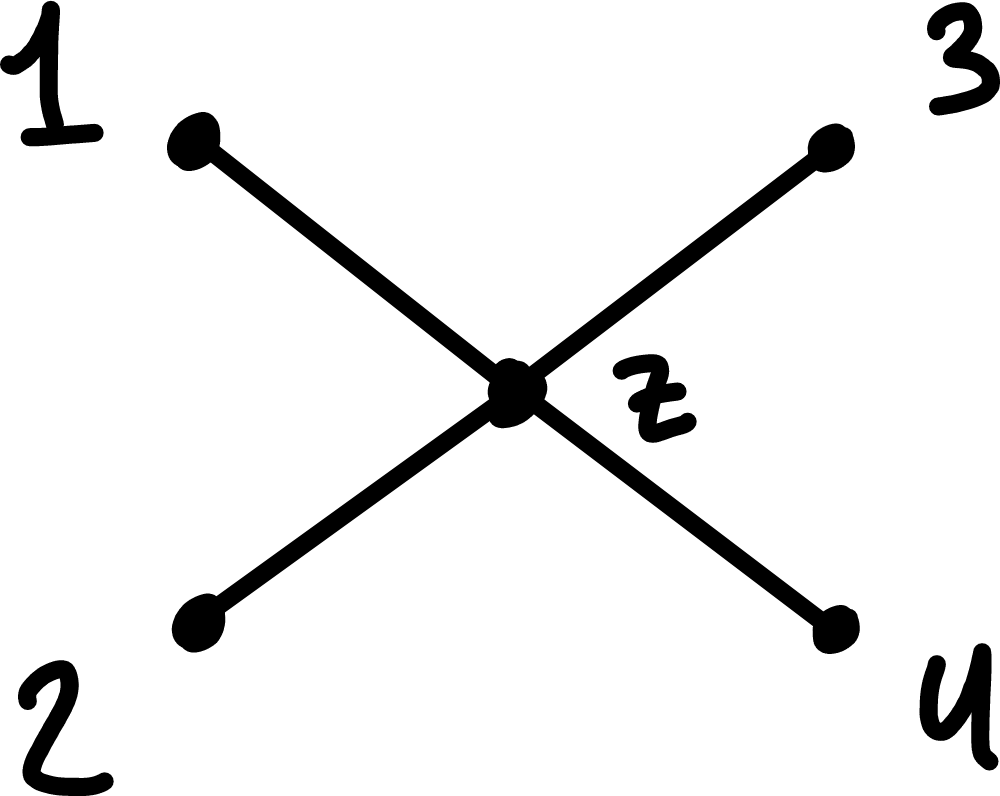
\includegraphics[width=0.3\textwidth]{Notewise-Untitled 2025-12-30-20260202134231.png}
    \caption{The only treelike Feynman diagram of first order in $\lambda$.}
\end{figure}
\newline
In all permutations of $G_4$ two of the fields interact with $\varphi(z)$ and two of the fields interact with $\varphi^*(z)$. There are $4$ options to each of the six permutations (two for the ambiguity in $\varphi(z)$ and two for the ambiguity in $\varphi^*(z)$):
\begin{equation}
\begin{gathered}
    G_4(x_1, x_2, x_3, x_4) = -i 4 \lambda \int d^4z G_2(x_1, z) G_2(x_2, z) G_3(x_3, z) G_3(x_4, z) + \\ +
    G_2(x_1, z) G_3(x_2, z) G_2(x_3, z) G_3(x_4, z) +
    G_2(x_1, z) G_3(x_2, z) G_3(x_3, z) G_2(x_4, z) + \\ +
    G_3(x_1, z) G_2(x_2, z) G_2(x_3, z) G_3(x_4, z) +
    G_3(x_1, z) G_2(x_2, z) G_3(x_3, z) G_2(x_4, z) + \\ +
    G_3(x_1, z) G_3(x_2, z) G_2(x_3, z) G_2(x_4, z)
\end{gathered}
\end{equation}
Each of these becomes a sum or a substraction of $D_F^{(n)}$s as we found. To make it easier to write, let us name:
\begin{equation}
    D_F^{(n)}(x_m - z) \equiv (m;n)
\end{equation}
And then, for example:
\begin{equation}
    G_2(x_1, z) = (1;1) + (2;1)
    \qquad
    G_3(x_1, z) = (1;1) - (2;1)
\end{equation}
This makes the above expression into:
\begin{equation}
\begin{gathered}
    G_4(x_1, x_2, x_3, x_4) = -i 4 \lambda \int d^4z \\
    \ \ [(1;1) + (2;1)] [(1;2) + (2;2)] [(1;3) - (2;3)] [(1;4) - (2;4)] + \\ +
    [(1;1) + (2;1)] [(1;2) - (2;2)] [(1;3) + (2;3)] [(1;4) - (2;4)] + \\ +
    [(1;1) + (2;1)] [(1;2) - (2;2)] [(1;3) - (2;3)] [(1;4) + (2;4)] + \\ +
    [(1;1) - (2;1)] [(1;2) + (2;2)] [(1;3) + (2;3)] [(1;4) - (2;4)] + \\ +
    [(1;1) - (2;1)] [(1;2) + (2;2)] [(1;3) - (2;3)] [(1;4) + (2;4)] + \\ +
    [(1;1) - (2;1)] [(1;2) - (2;2)] [(1;3) + (2;3)] [(1;4) + (2;4)] \ \
\end{gathered}
\end{equation}
Now it's clear to see that the there are $2^4$ combinations, but half of them do not survive. In each term there are four factors, one for each $x_n$. In each factor we sum over both fields, so we can sum by taking first all the terms where $\phi_2$ doesn't appear, and there is only $\phi_1$, then all the terms where $\phi_2$ appears once, then all terms where $\phi_2$ appears twice, and so forth. In the terms where there is only $\phi_1$, all terms look the same, and there are six of them:
\begin{equation}
    6(1;1)(1;2)(1;3)(1;4)
\end{equation}
In the terms where $\phi_2$ appears once, it is clear that there are always three positive terms and three negative terms, so they all cancel out. In terms where $\phi_2$ appears twice, there are four negative terms and two positive terms, resulting in a factor $-2$ to all such terms. Then, taking the terms where $\phi_2$ appears three times, they again cancel out, and then taking the terms where only $\phi_2$ appears, all six are positive. The total result is:
\begin{equation}
\begin{gathered}
    G_4(x_1, x_2, x_3, x_4) = -i 4 \lambda \int d^4z \\
    6 \left[D_F^{(1)}(x_1 - z)D_F^{(1)}(x_2 - z)D_F^{(1)}(x_3 - z)D_F^{(1)}(x_4 - z) + D_F^{(2)}(x_1 - z)D_F^{(2)}(x_2 - z)D_F^{(2)}(x_3 - z)D_F^{(2)}(x_4 - z)\right] - \\ -
    2[
        D_F^{(1)}(x_1 - z)D_F^{(1)}(x_2 - z)D_F^{(2)}(x_3 - z)D_F^{(2)}(x_4 - z) +
        D_F^{(1)}(x_1 - z)D_F^{(2)}(x_2 - z)D_F^{(1)}(x_3 - z)D_F^{(2)}(x_4 - z) + \\ +
        D_F^{(2)}(x_1 - z)D_F^{(1)}(x_2 - z)D_F^{(1)}(x_3 - z)D_F^{(2)}(x_4 - z) +
        D_F^{(1)}(x_1 - z)D_F^{(2)}(x_2 - z)D_F^{(2)}(x_3 - z)D_F^{(1)}(x_4 - z) + \\ +
        D_F^{(2)}(x_1 - z)D_F^{(1)}(x_2 - z)D_F^{(2)}(x_3 - z)D_F^{(1)}(x_4 - z) +
        D_F^{(2)}(x_1 - z)D_F^{(2)}(x_2 - z)D_F^{(1)}(x_3 - z)D_F^{(1)}(x_4 - z)
    ]
\end{gathered}
\end{equation}
This result seems big, but it's actually not surprising. We can see that the first two terms are terms where only one field interacts, while the second four terms include both fields. Moreover, in all terms, the number of particles of boths kinds remaind constant. This is the result of the conserved charge we saw earlier.
\newline
The process for $G_5$ is rather similar. The key difference is that instead of contracting either $\varphi\varphi$ or $\varphi^*\varphi$, we contract either $\varphi^*\varphi^*$ or $\varphi^*\varphi$. We still need all external fields to contract with $z$, to avoid loops. But, let us notice that
\begin{equation}
    \bra{0}\varphi^*(x)\varphi^*(y)\ket{0} = \bra{0}(\phi_1(x) - i\phi_2(x))(\phi_1(y) - i\phi_2(y))\ket{0} = D_F^{(1)}(y - x) - D_F^{(2)}(y - x) = G_3(x, y)
\end{equation}
So, we will get exactly the same combinations as in $G_4$, and thus the exact same result.

\subsection{Scattering matrix element}
Let us now find the scattering matrix element for the creationg of two $\phi_2$ particles from two $\phi_1$ particles:
\begin{equation}
    M(\phi_1(p) + \phi_1(p') \rightarrow \phi_2(k) + \phi_2(k'))
\end{equation}
To do this, let us look at the correlation function $\bra{\Omega}T\phi_1(x_1)\phi_1(x_2)\phi_2(y_1)\phi_2(y_2)\ket{\Omega}$. First, let us write the interaction term in terms for $\phi_1$ and $\phi_2$:
\begin{equation}
    \mathcal{L}_{int} = -\lambda(\varphi^*\varphi)^2 - \lambda(\phi_1^2 + \phi_2^2)^2 = -\lambda(\phi_1^4 + \phi_2^4 - 2\phi_1^2\phi_2^2)
\end{equation}
So, the relevant interaction term is $2\lambda\phi_1^2\phi_2^2$, since it is the one that can be contracted with two particles of each type. The correlation function is then (to first order in $\lambda$):
\begin{equation}
    \bra{\Omega}T\phi_1(x_1)\phi_1(x_2)\phi_2(y_1)\phi_2(y_2)\ket{\Omega} =
    -2i\lambda \int d^4z \bra{0}T\phi_1(x_1)\phi_1(x_2)\phi_2(y_1)\phi_2(y_2)\phi_1(z)\phi_1(z)\phi_2(z)\phi_2(z)\ket{0}
\end{equation}
Using Wick's theorem, we contract each field with its own type. There are two options for the connection of each field, leading to 4 total permutations:
\begin{equation}
    G_{11\rightarrow22} = \bra{\Omega}T\phi_1(x_1)\phi_1(x_2)\phi_2(y_1)\phi_2(y_2)\ket{\Omega} = -8i\lambda \int d^4z D_F^{(1)}(x_1 - z) D_F^{(1)}(x_2 - z) D_F^{(2)}(z - y_1) D_F^{(2)}(z - y_2)
\end{equation}
Fourier transforming it (flipping the momentum constants to match the direction of the propagator, and naming $x_{3,4} = y_{1,2}$ for convinience of indices, as well as $p_{1,2,3,4} = p, p', k, k'$):
\begin{equation}
\begin{gathered}
    \tilde{G}_{11\rightarrow22} = -8i\lambda \int d^4z \int e^{-ipx_1} d^4x_1 \int  e^{-ip'x_2} d^4x_2 \int e^{iky_1} d^4y_1 \int e^{ik'y_2} d^4y_2 \prod_{j=1,\dots,4} \int \frac{d^4k_j}{(2\pi)^4}\frac{ie^{-ik_j(x_j - z)}}{k_j^2 - m_1^2 + i\varepsilon} = \\ =
    -8i\lambda \prod_{j=1,\dots,4} \frac{i}{k_j^2 - m_1^2 + i\varepsilon} \int d^4z e^{-iz(p + p' - (k + k'))} = \\ =
    -8i\lambda \prod_{j=1,\dots,4} \frac{i}{k_j^2 - m_1^2 + i\varepsilon} (2\pi)^4\delta(p + p' - k - k')
\end{gathered}
\end{equation}
This matches the formulation of the $2 \rightarrow 2$ LSZ formula, which means that
\begin{equation}
    M_{11 \rightarrow 22} = -8\lambda
\end{equation}
\newpage
\section{Effective theory with Dirac Fermions}
Looking at the Dirac fermion $\psi$ and the real scalar field $\phi$ with the Lagrangian density:
\begin{equation}
    \mathcal{L} = \bar{\psi}(i\slashed{\partial} - m)\psi + \frac{1}{2}\partial_\mu\phi \partial^\mu \phi - \frac{M^2}{2}\phi^2 - ig\phi\bar{\psi}\gamma^5\psi
\end{equation}
\subsection{Properties of the Lagrangian}
\subsubsection{The last term is a scalar}
Since $\phi$ is a scalar, it is invariant under Lorentz transformation:
\begin{equation}
    \phi \rightarrow \phi' = \phi
\end{equation}
While $\psi$ transforms according to the transformation of Dirac spinors:
\begin{equation}
    \psi = \begin{pmatrix}
        \psi_L \\ \psi_R
    \end{pmatrix} \rightarrow \psi' = \begin{pmatrix}
        \psi_L' \\ \psi_R'
    \end{pmatrix} = \begin{pmatrix}
        M_L\psi_L \\ M_R\psi_R
    \end{pmatrix}
\end{equation}
Where
\begin{equation}
    M_{L,R} = e^{-i(\theta_\alpha \pm iy_\alpha)\frac{1}{2}\sigma_\alpha}
\end{equation}
are the transformations for the lefthanded and righthanded Weyl spinors making up the Dirac spinor. So, this gives:
\begin{equation}
\begin{gathered}
    \bar{\psi}\gamma^5\psi \rightarrow \bar{\psi}'\gamma^5\psi' =
    \begin{pmatrix}
        \psi_R^\dagger M_R^\dagger & \psi_L^\dagger M_L^\dagger
    \end{pmatrix}
    \begin{pmatrix}
        -\mathbb{I}_{2\times2} & \\ & \mathbb{I}_{2\times2}
    \end{pmatrix}
    \begin{pmatrix}
        M_L\psi_L \\ M_R\psi_R
    \end{pmatrix}
    = \\ =
    - \psi_R^\dagger M_R^\dagger M_L\psi_L + \psi_L^\dagger M_L^\dagger M_R\psi_R
\end{gathered}
\end{equation}
Noticing that since $\sigma_\alpha$ are hermitian:
\begin{equation}
    M_{L, R}^\dagger = e^{i(\theta_\alpha \mp iy_\alpha)\frac{1}{2}\sigma_\alpha} = M_{R,L}^{-1}
\end{equation}
We get:
\begin{equation}
\begin{gathered}
    \bar{\psi}'\gamma^5\psi' = - \psi_R^\dagger M_R^\dagger M_L\psi_L + \psi_L^\dagger M_L^\dagger M_R\psi_R = - \psi_R^\dagger \psi_L + \psi_L^\dagger \psi_R = \\ =
    \begin{pmatrix}
        \psi_R^\dagger & \psi_L^\dagger
    \end{pmatrix}
    \begin{pmatrix}
        -\mathbb{I}_{2\times2} & \\ & \mathbb{I}_{2\times2}
    \end{pmatrix}
    \begin{pmatrix}
        \psi_L \\ \psi_R
    \end{pmatrix}
    = \bar{\psi}\gamma^5\psi
\end{gathered}
\end{equation}
And so, since $\bar{\psi}\gamma^5\psi$ transforms like a scalar, and $\phi$ transforms like a scalar, the last term $\phi\bar{\psi}\gamma^5\psi$ transforms like a scalar as well.
\subsubsection{The action is real}
It's obvious that the second and third terms are real, since they only include the real field. The first term, the free Dirac field, includes the mass term, which is again obviously real, and the kinetic term $i\bar{\psi}\slashed{\partial}\psi$. Let us show it is real in the action integral:
\begin{equation}
\begin{gathered}
    \left(\int d^4x i\bar{\psi}\slashed{\partial}\psi\right)^* = 
    \\ =
    \left(\int d^4x i \psi^\dagger \gamma^0 \gamma^\mu \partial_\mu \psi\right)^* = \\ =
    \left(\int d^4x i \psi^\dagger \gamma^{\mu\dagger}\gamma^0 \partial_\mu  \psi\right)^* = \\ =
    - \int d^4x i  \partial_\mu (\psi^\dagger) \gamma^0 \gamma^{\mu} \psi = \\ =
    \int d^4x i \psi^\dagger \gamma^0 \gamma^{\mu} \partial_\mu \psi + \ edge \ terms = \\ =
    \int d^4x i \bar{\psi} \slashed{\partial} \psi + \ edge \ terms =
\end{gathered}
\end{equation}
Where we used the identity $\gamma^0\gamma^\mu = \gamma^{\mu\dagger}\gamma^0$, and integrated by parts in the next to last transition.
\newline
Lastly, we need to show the same for the last term $ig\phi\bar{\psi}\gamma^5\psi$. Since $g\phi$ is real, we just need to show that $i\bar{\psi}\gamma^5\psi$ is real. Using the same method:
\begin{equation}
    (i\bar{\psi}\gamma^5\psi)^* = (i\psi^\dagger\gamma^0\gamma^5\psi)^* = -i\psi^\dagger\gamma^5\gamma^0\psi = i\psi^\dagger\gamma^0\gamma^5\psi = i\bar{\psi}\gamma^5\psi
\end{equation}

\subsubsection{Mass dimensions}
Since the action is dimensionless, the mass dimensions of the Lagrangian density is $\left[\mathcal{L}\right] = 4$. Using this, we can find the mass dimension of each of fields and parameters.
\newline
Starting from the scalar field, in the second term it appears twice with two derivatives. The mass dimension of each derivative is 1, so the field must also have a mass dimension $\left[\phi\right] = \frac{1}{2}(4 - 2) = 2$. The same can be extracted for the Dirac Fermion field, where it appears twice, but with a single derivative in its kinetic term. So, its mass dimension must be $\left[\psi\right] = \frac{1}{2}(4 - 1) = 1.5$
This also aligns with both mass constants $m$ and $M$.
\newline
Lastly, we can find the mass dimension of $g$ from the two fields. The total dimension of the last term is
\begin{equation}
    [g\phi\bar{\psi}\gamma^5\psi] = [g] + 1.5 + 1 + 1.5 = [g] + 4 = 4
\end{equation}
Therefore $[g] = 0$

\subsection{Full theory correlation function}
Let us look at the time correlation function
\begin{equation}
    G_{abcd}(x_1, x_2; y_1, y_2) \equiv \bra{\Omega}T \psi_a(x_1)\psi_b(x_2)\bar{\psi}_c(y_1)\bar{\psi}_d(y_2)\ket{\Omega}
\end{equation}
In order $g^2$, we allow two interactions, i.e. two vertices in the Feynman diagrams:
\begin{figure}[h]
    \centering
    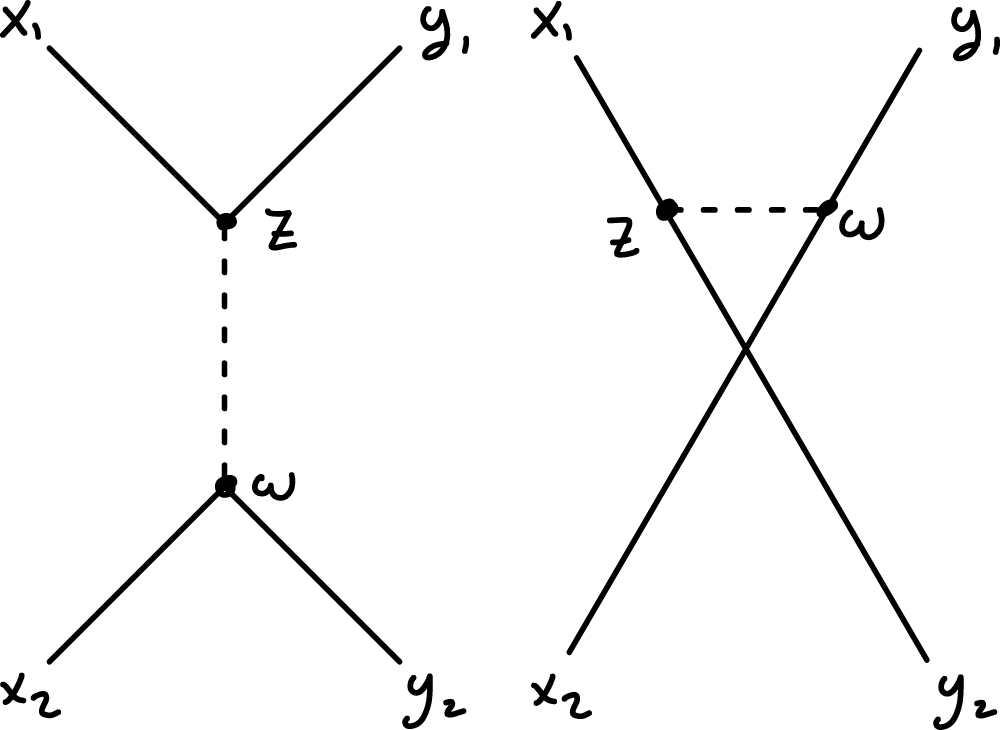
\includegraphics[width=0.5\textwidth]{Notewise-1000006698-20260331154044.png}
    \caption{The allowed Feynman diagrams for second order in $g$.}
\end{figure}
This becomes:
\begin{equation}
\begin{gathered}
    G_{abcd}(x_1, x_2; y_1, y_2) = \bra{0}T
        \psi_a(x_1)\psi_b(x_2)\bar{\psi}_c(y_1)\bar{\psi}_d(y_2)(-i)^2(-ig)^2\int d^4z\phi(z)\bar{\psi}(z)\psi(z)\int d^4w\phi(w)\bar{\psi}(w)\psi(w)
    \ket{0} = \\ =
    (-i)^2(-ig)^2\int d^4z\int d^4w\bra{0}T
        \psi_a(x_1)
        \psi_b(x_2)
        \bar{\psi}_c(y_1)
        \bar{\psi}_d(y_2)
        \phi(z)
        \bar{\psi}_e(z)
        \psi_f(z)
        \bar{\psi}_g(w)
        \psi_h(w)
    \ket{0}
\end{gathered}
\end{equation}
In each Dirac spinor field there are two Weyl spinors. In the interaction, they are interacting oppositly: the righthanded Weyl spinor from one field interacts with the lefthanded Weyl spinor from the other field and vice versa. This gives us two interactions, one for each such pair. Now, using wick's theorem, we get two permutations, one where $x_1$ and $y_1$ are contracted with a field of the same internal index, and one where $x_1$ and $y_2$ are contracted with a field of the same internal index. In each of those permutations we contract four fields, each contraction comes with a dummy index for the two possible internal spinor indices. At the end of the calculation we will need to impose the requirement that those indices match the interaction:
\begin{equation}
\begin{gathered}
    \sum_{efgh=R,L}
    \bra{0}T
        \psi_a(x_1)
        \psi_b(x_2)
        \bar{\psi}_c(y_1)
        \bar{\psi}_d(y_2)
        \phi(z)
        \bar{\psi}_e(z)
        \psi_f(z)
        \bar{\psi}_g(w)
        \psi_h(w)
    \ket{0} = \\ =
    \sum_{efgh=R,L}
        \contraction[0.5ex]{}{\psi_a}{(x_1)\psi_b(x_2)\bar{\psi}_c(y_1)\bar{\psi}_d(y_2)\phi(z)}{\bar{\psi}}
        \contraction{\psi_a(x_1)}{\psi_b}{(x_2)\bar{\psi}_c(y_1)\bar{\psi}_d(y_2)\phi(z)\bar{\psi}_e(z)\psi_f(z)}{\bar{\psi}}
        \contraction{\psi_a(x_1)\psi_b(x_2)}{\bar{\psi}_c}{(y_1)\bar{\psi}_d(y_2)\phi(z)\bar{\psi}_e(z)}{\psi}
        \contraction[1.5ex]{\psi_a(x_1)\psi_b(x_2)\bar{\psi}_c(y_1)}{\bar{\psi}_d}{(y_2)\phi(z)\bar{\psi}_e(z)\psi_f(z)\bar{\psi}_g(z)}{\psi}
        \psi_a(x_1)
        \psi_b(x_2)
        \bar{\psi}_c(y_1)
        \bar{\psi}_d(y_2)
        \phi(z)
        \bar{\psi}_e(z)
        \psi_f(z)
        \bar{\psi}_g(w)
        \psi_h(w) +
        \contraction[0.5ex]{}{\psi_a}{(x_1)\psi_b(x_2)\bar{\psi}_c(y_1)\bar{\psi}_d(y_2)\phi(z)}{\bar{\psi}}
        \contraction{\psi_a(x_1)}{\psi_b}{(x_2)\bar{\psi}_c(y_1)\bar{\psi}_d(y_2)\phi(z)\bar{\psi}_e(z)\psi_f(z)}{\bar{\psi}}
        \contraction{\psi_a(x_1)\psi_b(x_2)}{\bar{\psi}_c}{(y_1)\bar{\psi}_d(y_2)\phi(z)\bar{\psi}_e(z)\psi_f(z)\bar{\psi}_g(z)}{\psi}
        \contraction[1.5ex]{\psi_a(x_1)\psi_b(x_2)\bar{\psi}_c(y_1)}{\bar{\psi}_d}{(y_2)\phi(z)\bar{\psi}_e(z)}{\psi}
        \psi_a(x_1)
        \psi_b(x_2)
        \bar{\psi}_c(y_1)
        \bar{\psi}_d(y_2)
        \phi(z)
        \bar{\psi}_e(z)
        \psi_f(z)
        \bar{\psi}_g(w)
        \psi_h(w)
\end{gathered}
\end{equation}
We can notice that in the second permutation the two fields at point $z$ must switch places in order to contract with their matching fields. This gives the second term a minus sign from the anticommutation of fermions, resulting in:
\begin{equation}
\begin{gathered}
    G_{abcd}(x_1, x_2; y_1, y_2) = g^2 \int d^4z \int d^4 w D_F(z - w) \\ \sum_{efgh=R,L}\left[S_{Fae}(x_1 - z)S_{Fcf}(y_1 - z)S_{Fbg}(x_2 - w)S_{Fdh}(y_2 - w) - S_{Fae}(x_1 - z)S_{Fdf}(y_2 - z)S_{Fbg}(x_2 - w)S_{Fch}(y_1 - w)\right]
\end{gathered}
\end{equation}
Now, noticing how the interactions change the spinor index, we must require that the spinor propagators meeting at the same vertex will have opposite spinor indices, marked using $e = \bar{f}$:
\begin{equation}
\begin{gathered}
    G_{abcd}(x_1, x_2; y_1, y_2) = g^2 \int d^4z \int d^4 w D_F(z - w) \\ \sum_{fg=R,L}\left[S_{Fa\bar{f}}(x_1 - z)S_{Fcf}(y_1 - z)S_{Fbg}(x_2 - w)S_{Fd\bar{g}}(y_2 - w) - S_{Fa\bar{f}}(x_1 - z)S_{Fdf}(y_2 - z)S_{Fbg}(x_2 - w)S_{Fc\bar{g}}(y_1 - w)\right]
\end{gathered}
\end{equation}

\subsection{A simplified theory}
Let us now take $M$ to be very large.
\subsubsection{The EOM for $\phi$}
Using Euler Lagrange:
\begin{equation}
    \frac{\partial \mathcal{L}}{\partial\phi} = -M^2\phi - ig\bar{\psi}\gamma^5\psi
    \qquad
    \partial^\mu \frac{\partial \mathcal{L}}{\partial\left(\partial^\mu \phi\right)} = \partial^\mu\partial_\mu \phi = \Box \phi
\end{equation}
So, this gives:
\begin{equation}
    \Box \phi = - M^2\phi - ig\bar{\psi}\gamma^5\psi
\end{equation}
\begin{equation}
    \left(\Box + M^2\right) \phi = - ig\bar{\psi}\gamma^5\psi
\end{equation}
We notice that this equation, when $g \rightarrow 0$, becomes the Klein Gordon equation for a free scalar field.
\subsubsection{A perturbative solution}
We can now exapnd the field in powers of $1/M^2$. In first order we can simply neglect the derivative $\partial_\mu$:
\begin{equation}
    \left(\Box + M^2\right) \phi_0 = - ig\bar{\psi}\gamma^5\psi \rightarrow \phi_0 = -i\frac{g}{M^2}\bar{\psi}\gamma^5\psi
\end{equation}
Up to next it is then
\begin{equation}
    \phi = -i\frac{g}{M^2}\bar{\psi}\gamma^5\psi + \frac{1}{M^4}\phi_1
\end{equation}
Plugging this into the equation gives:
\begin{equation}
    \left(\Box + M^2\right)\left(-i\frac{g}{M^2}\bar{\psi}\gamma^5\psi + \frac{1}{M^4}\phi_1\right) = -i\frac{g}{M^2}\Box\bar{\psi}\gamma^5\psi + \frac{1}{M^4}\Box\phi_1 - ig\bar{\psi}\gamma^5\psi + \frac{1}{M^2}\phi_1 = - ig\bar{\psi}\gamma^5\psi
\end{equation}
Therefore (now taking to order $1/M^2$):
\begin{equation}
    -i\frac{g}{M^2}\Box\bar{\psi}\gamma^5\psi + \frac{1}{M^2}\phi_1 = 0
\end{equation}
\begin{equation}
    \phi_1 = ig\Box\bar{\psi}\gamma^5\psi
\end{equation}
Which means the next correction is of order $1/M^4$.
\subsubsection{The new Lagrangian}
Substituting back into the Lagrangian density gives:
\begin{equation}
    \mathcal{L}_{eff} = \bar{\psi}(i\slashed{\partial} - m)\psi - \frac{g^2}{2M^4}\partial_\mu(\bar{\psi}\gamma^5\psi) \partial^\mu (\bar{\psi}\gamma^5\psi) + \frac{g^2}{2M^2}(\bar{\psi}\gamma^5\psi)^2 - \frac{g^2}{M^2}(\bar{\psi}\gamma^5\psi)^2
\end{equation}
Taking up to first order in $1/M^2$, we get:
\begin{equation}
    \mathcal{L}_{eff} = \bar{\psi}(i\slashed{\partial} - m)\psi + c(\bar{\psi}\gamma^5\psi)^2
    \qquad
    c = -\frac{g^2}{2M^2}
\end{equation}

\subsection{Interactions in the effective theory}
Let us now look again at $G_{abcd}(x_1, x_2 ; y_1, y_2)$, but in the new theory, up to first order in $c$. There are two options for contraction of each field, in total four options, two of which have to get a minus sign because of the Grassman property of the fields. Again, like in the full theory, we get a sum over spinor indices, but in this case since there are four Dirac fields in the interaction, which means there can be two pairs of opposite spins. This gives us another factor of 2 for the two different configuration of spin indices exiting the interaction vertex. But, we must notice that these permutations conincide with the permutations over the fields themselves, so the total factor is 2:
\begin{equation}
\begin{gathered}
    G_{abcd}(x_1, x_2 ; y_1, y_2) = \sum_{efgh=R,L}
    \bra{0}T\psi_a(x_1)\psi_b(x_2)\bar{\psi}_c(y_1)\bar{\psi}_d(y_2)(-ic)\int d^4z\psi_e(z)\bar{\psi}_f(z)\psi_g(z)\bar{\psi}_h(w)\ket{0} = \\ =
    - 2ic \sum_{fg=R,L}
    \int d^4z \\ \left[S_{Faf}(x_1 - z)S_{Fc\bar{f}}(y_1 - z)S_{Fbg}(x_2 - z)S_{Fd\bar{g}}(y_2 - z) - S_{Faf}(x_1 - z)S_{Fd\bar{f}}(y_2 - z)S_{Fbg}(x_2 - z)S_{Fc\bar{g}}(y_1 - z)\right]
\end{gathered}
\end{equation}

\subsection{Equivilance}
The two expression we got in the two theories are equivilant. To see that, we can write $g^2 = -2M^2c$ and see how in the first expression we get:
\begin{equation}
\begin{gathered}
    g^2 D_F(z-w) = -2M^2c \int \frac{d^4k}{(2\pi)^4}\frac{ie^{-ik(z - w)}}{k^2 - M^2 + i\varepsilon} = \\ =
    2ic \int \frac{d^4k}{(2\pi)^4}\frac{e^{-ik(z - w)}}{1 - \frac{k^2}{M^2} + i\varepsilon} \approx 2ic \int \frac{d^4k}{(2\pi)^4}\left(e^{-ik(z - w)}\right) \\ = 2ic\delta(z - w)
\end{gathered}
\end{equation}
Which when assigned back into the expression gives (up to a sign) the result from the effective theory.
\end{document}